%
%   K A D O N O
%   "kadono.tex"
%

\documentclass[10pt,b5paper,papersize,dvipdfmx]{jsbook}

\usepackage{vuccaken}
\usepackage{vuccaken2019}

% スタイルファイルの読み込みや自作マクロは、
% 最終的には vuccaken2019.sty の中に書いてください。
% とりあえずはここに書いてもらって構いません。


\begin{document} % 以下本文

% \mokuji{2} % 目次出力

% - - - - - - - - - - - - - - - - - - - - - - - - %
\kaishititle%
  {温度の子}% title
  {基礎理工学研究科 M 1回生}% 所属
  {\vname{門野}{広大}}% name
% - - - - - - - - - - - - - - - - - - - - - - - - %


\section*{はじめに}
熱って何?温度ってなに?どうやって熱は伝わっているの?そんな疑問に一生に一度は出会ったことがあると思います。実際熱の伝わり方というものをちゃんと理解しようとすると莫大な時間がかかりますし、不可逆なものでもあるのでそもそも理解できないのかもしれません。でも、限定的な条件において理解することは容易にできます。今回の会誌ではそんな物理の世界では常識的なことを主に書いていきたいと思います。\par
今回は状況が限定的な状態で、実際に人間が住んでいる環境とはかけ離れているため役に立たないと思われると思います。研究分野ではとても役にたちます。その理由を最後の方に私がやっている研究の話を含めて書きたいと思います。

% 熱って何?そもそも温度って何?熱伝導率って何で決まるの?物質のなに?格子ってなに?
% 格子振動って何?フォノンってなに?

%
\section{温度}
温度とは、辞書で検索すると「温冷の度合いを表す指標である」と書いてあります。その通りなんですけど、状態量として使われているので、そもそもどういう形で決まっているのか気になると思います。私は今回この会誌を書くに当たってとても気になりました。\par 
普段日本人なら$^\circ \rm{C}$という単位の世界で過ごしていると思います。これはセルシウス度というものらしいです。水を冷やしていったときに氷になる温度を$0 ^\circ \rm{C}$として、水を温めていったときに沸騰する温度を$100 ^\circ \rm{C}$と決めた温度だそうです。ほかにもいろんな温度があるらしいですが、今回使う温度の単位は$\rm{K}$です。高校の物理でもやると思うので知っている人は多いと思いますが、読み方はケルビンです。このケルビンは国際単位系で熱力学温度の単位になっています。\par
ケルビンが何を基準にしているのかを考える前に、温度というものはミクロの世界で考えるとどういうものに対応するのかということを考えていきましょう。統計力学の教科書を読むと物質を構成する分子がもつエネルギーの統計値である、と書いてあります\par
絶対温度はほかの状態量の中で測定するがかなり難しいです。実際に大学の研究室で試料の温度を測定するときに使用している温度計はいろんな種類がありますが、その中の一つはセルノックス温度センサーです。私も実際に実験で使用しました。この温度計は温度が上がると抵抗値が下がるという負の温度係数を持っています。
\begin{figure}[htbp]
  \begin{center}
      \begin{tabular}{c}
      % 1
      \begin{minipage}{0.5\hsize}
          \begin{center}
          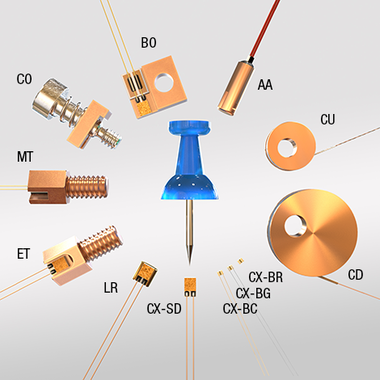
\includegraphics[clip, width=4.5cm]{kadono/cryotronics.png}
          \hspace{1.6cm} [A]\ セルノックス温度センサ
          \end{center}
      \end{minipage}
      % 2
      \begin{minipage}{0.5\hsize}
          \begin{center}
          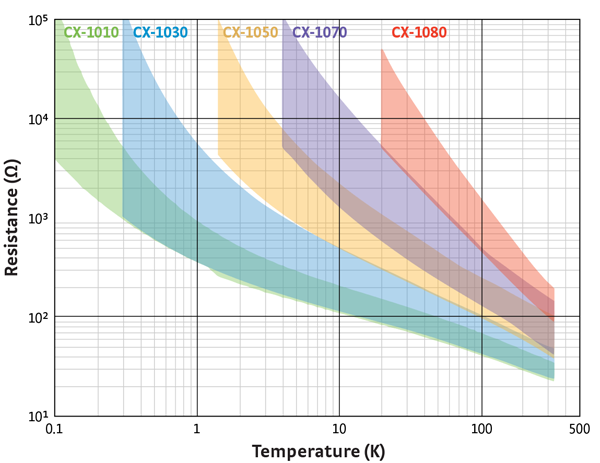
\includegraphics[clip, width=6cm]{kadono/CXチャート1.png}
          \hspace{1.6cm} [B]\ センサーの抵抗温度特性
          \end{center}
      \end{minipage}
  
      \end{tabular}
      \caption{セルノックス温度センサ、参考文献\cite{ondo}より}
      \label{fig:cryotronics}
  \end{center}
\end{figure}
セルノックス温度計の大きさは図\ref{fig:cryotronics}の[A]にある通りとて小さいです。セルノックスは低温特に数ケルビンの極低温領域に強い温度計です。摂氏でいうと$-270\ ^\circ \rm{C}$付近です。\ref{fig:cryotronics}の[B]にセルノックスの温度と抵抗値の特性をのせています。色の違いは種類の違いです。このグラフを見ると温度と抵抗値のグラフが直線ではなく幅を持っています。これはセルノックスの温度計自体にこれだけの抵抗値の誤差があるということではありません。個体差がこれくらいの幅を持っているということです。この温度計を買うとものと一緒に温度と抵抗値のデータがついてきます。このデータは企業側が測定してくれたデータです。このデータを使って校正することによって温度を正確に測定することができます。というように、絶対温度を測定するのは難しくどうしても相対温度を測定することになってしまいます。

\section{フォノン君}
今回は気体、液体ではなく、固体の中の熱の流れについて考えようと思います。
\subsection{格子振動}
まず考えたいのが、固体の中でも、一つの原子のみで構成されている単結晶です。
最初から三次元で考えるとよくわからなくなるので、原子同士がばねで一列につながっている状態を考えます(図\ref{fig:bane})。\par

\begin{figure}[htbp]
  \centering
  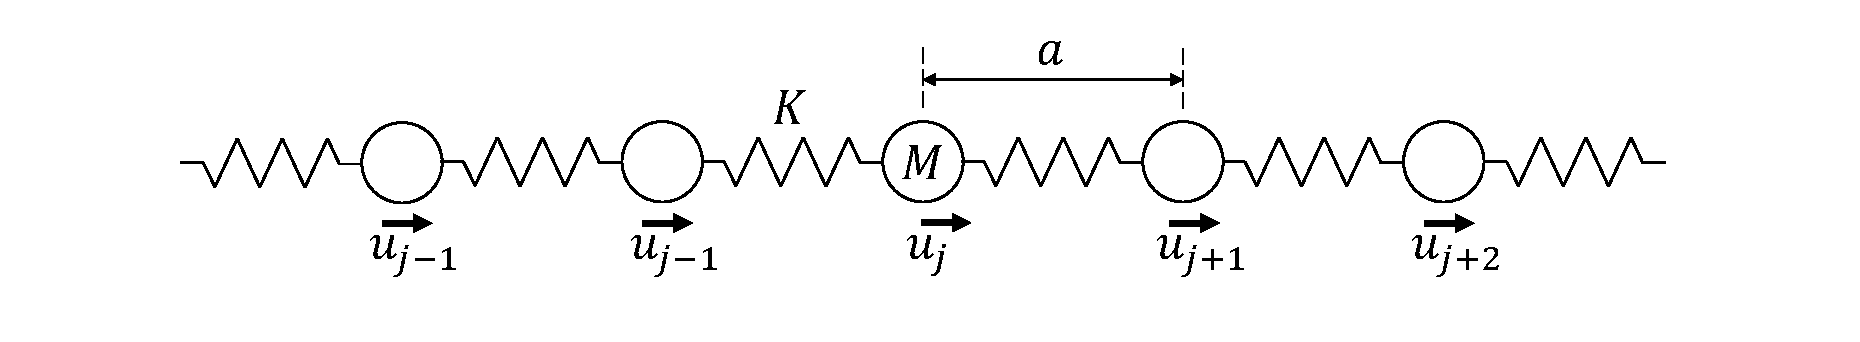
\includegraphics[height=2cm]{kadono/bane.pdf}  % width
  \caption{一次元の結晶}
  \label{fig:bane}
\end{figure}
構成原子は最近接の間にだけ力を及ぼし会うと仮定します。$s$番目の原子の変位を$u_s$すると、$s$番目の原子の運動方程式は次のようにあらわされる。
\begin{align}
  M\frac{\mathrm{d}^2u_s}{\mathrm{d}t^2} = F_s = \alpha (u_{s+1} - u_s) - \alpha (u_s - u_{s-1})
  \label{eq:satom}
\end{align}
ここで、$M$は原子の質量、$\alpha$はばね定数、$F_s$は$s$番目の原子に及ぼす力。\par
式\ref{eq:satom}の解は波の式であると予測されます。波の式について少し話をしましょう。代表的な正弦波をあらわす式は
\begin{align}
  A(x) = A_0 \sin \left(\frac{2\pi x}{\lambda} + \phi \right)
\end{align}
とかけます。\par
ここで、波数$k$というものを導入すると、
\begin{align}
  A(x) = A_0 \sin (kx + \phi)
\end{align}
となります。波数$k (= 2\pi/\lambda)$は、単位長さあたりに含まれる1波長分の波の数に$2\pi$をかけた量である。さあ、ここで波数$k$というものをわざわざ導入しました。どうしてこんなものを導入するのか疑問に思う人がいると思います。大学では友達以上にであう波数$k$がどういうものを示しているのでしょうか。\par
この波数が波の進行方向を含んだ波数ベクトル$\bm{k}$という形にして、空間波の式は次のようになる。
\begin{align}
  u(\bm{r},t) = u_0 \exp(i(\bm{k} \cdot \bm{r} - \omega t))
\end{align}
ここで、$u_0$は振幅、$\bm{k}$は波数ベクトル、$\bm{r}$は位置ベクトル、$\omega$は角周波数。\par

したがって、角振動数$\omega$と波数$\bm{k}$の関係には次のような関係がある。
\begin{align}
  \omega = 2 \sqrt{\frac{K}{M}} \left| \sin \frac{ka}{2}\right|
\end{align}
いろいろあって分散関係がでます。

\subsection{量子化}
量子力学によると、すべてのものは粒子と波の二重性を示すらしいです。この考えを今回の格子振動に適用して、粒子として考えることができます。この粒子のことをフォノン(phonon)と言います。


\section{比熱とか熱伝導率とか}
ここからは、固体中の熱物性、特に比熱、熱伝導率、について書いていきたいと思います。
\subsection{比熱}
比熱について、まず比熱とは、1 kgの物質の温度を1 Kだけあげるのに必要な熱量として定義されいます。水の場合、比熱は$4.2 \times 10^3\  \mathrm{J\ K ^{-1} kg^{-1}}$なので、1 kgの水の温度を1 Kあげるためには$4.2 \times 10^3 J$だけの熱量が必要ということになります。これに対して、銅の比熱は$3.8 \times 10^2\ \mathrm{J\ K ^{-1} kg^{-1}}$と水の比熱の1/10以下である。つまり、銅の方が水よりも10倍温まりやすい。\par
固体の比熱について考えるためには統計力学の知識が必要ですが、それは参考文献に任せて次に進みます。比熱は、$\frac{\mathrm{d}U}{\mathrm{d}T}$
\subsection{熱伝導率}
\section{ちょっと変わった話}
結晶において低温の熱物性について考えて来ました。前のセクションでいった温度依存性がすべての結晶でいえるのかというと実は例外があります。私の研究テーマになっているのですが、単結晶であってもなぜか結晶とは違う温度依存性を持つ物質がこの世の中には存在しています。リラクサー強誘電体というものです。

\begin{figure}[htbp]
  \begin{center}
      \begin{tabular}{c}  
      \begin{minipage}{0.5\hsize}
          \begin{center}
          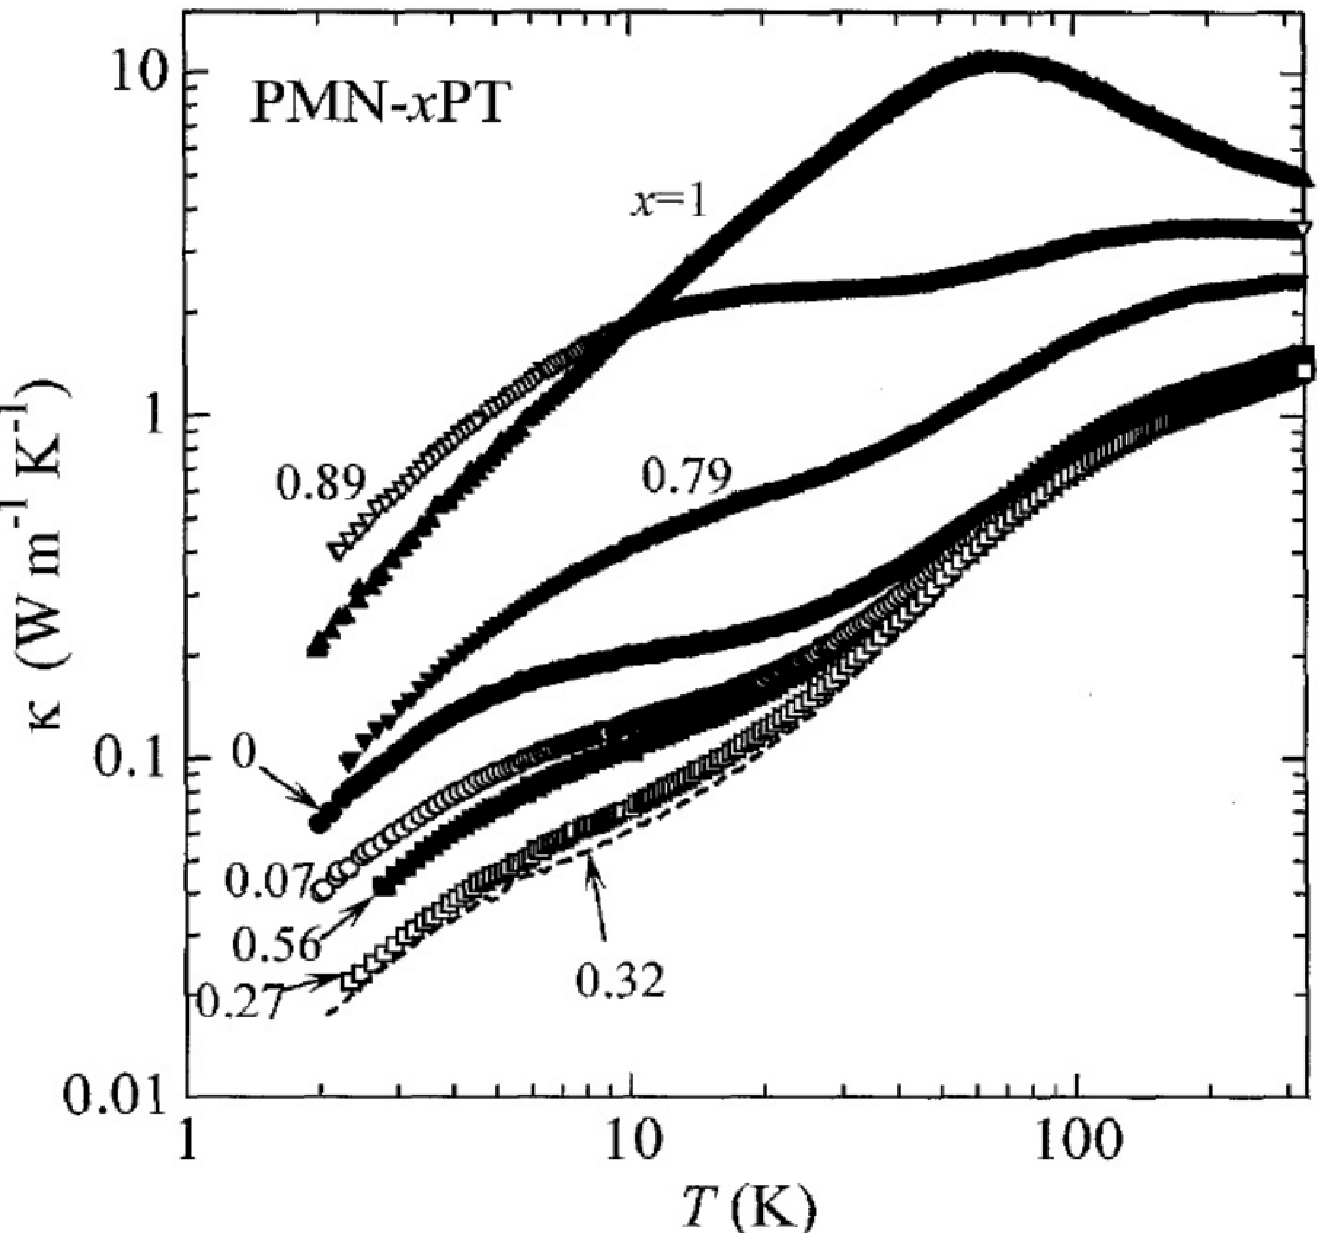
\includegraphics[clip, width=6cm]{kadono/リラクサー熱伝導率.pdf}
          \hspace{1.6cm} [A]熱伝導率の温度依存性
      \end{center}
  \end{minipage}
  \begin{minipage}{0.5\hsize}
      \begin{center}
          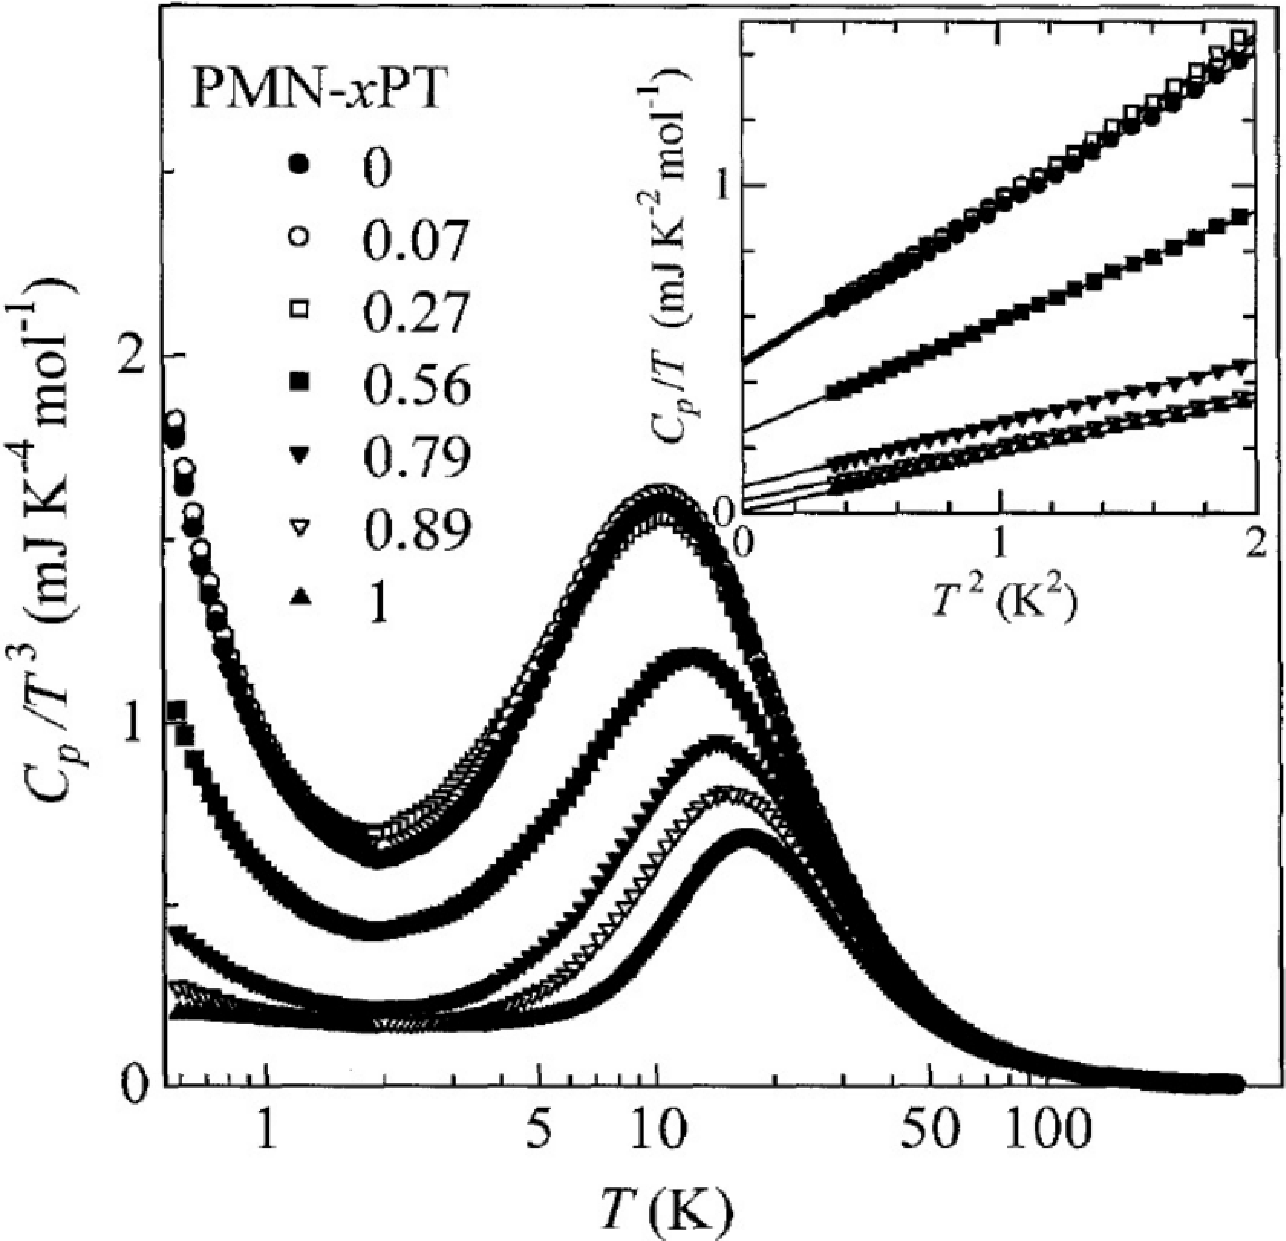
\includegraphics[clip, width=6cm]{kadono/リラクサー比熱.pdf}
          \hspace{1.6cm} [B]比熱の温度依存性
      \end{center}
      \end{minipage}
      \end{tabular}
      \caption{PMN-$x$PTのガラス的な熱物性\cite{relaxCT}}
      \label{fig:lena}
  \end{center}
\end{figure}
\section{終わりに}
% \begin{figure}[htbp]
%   \centering
%   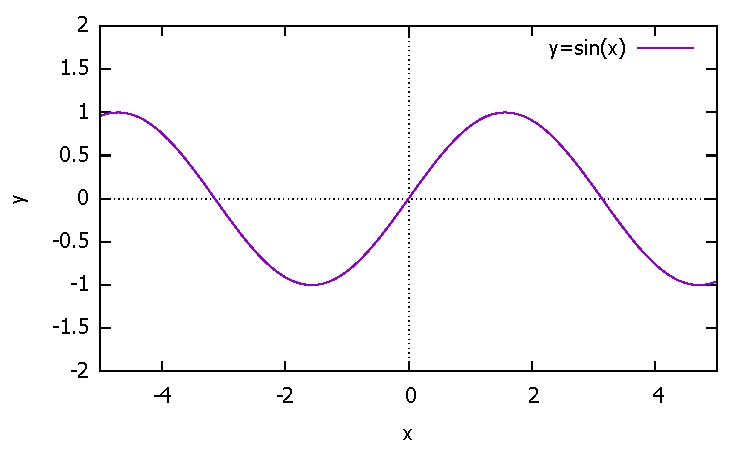
\includegraphics[width=10cm]{temp/fig-sin.pdf}
%   \caption{$y=\sin x$のグラフ。gnuplotで作成した。}
%   \label{fig:sin}
% \end{figure}

%% 参考文献
\begin{thebibliography}{99}
  \bibitem{ondo} \url{https://www.toyo.co.jp/material/products/detail/id=648}
  \item 横田伊佐秋,『物理学テキストシリーズ 熱力学』,岩波書店,1987.
  \item 矢口裕之,『初歩から学ぶ固体物理学』,講談社,2017.
  \item W.COCHRAN・小林正一・福地充(訳),『固体物性シリーズ3 格子振動』,丸善出版,昭和50年.
  \item 田崎晴明,『新物理学シリーズ37 統計力学』,培風館,2008.
  \item 相沢洋二,『キーポイント熱・統計力学』,岩波書店,1996.
 \bibitem{relaxCT}
  Tachibana et al, Appl. Phys. Lett, 93, 092902 (2008).
\end{thebibliography}

\end{document}
%
% ファイトだよ!
%